\let\negmedspace\undefined
\let\negthickspace\undefined
\documentclass[journal]{IEEEtran}
\usepackage[a5paper, margin=9mm, onecolumn]{geometry}
\usepackage{lmodern} 
\usepackage{tfrupee} 

\setlength{\headheight}{1cm} 
\setlength{\headsep}{0mm}     

\usepackage{gvv-book}
\usepackage{gvv}
\usepackage{cite}
\usepackage{amsmath,amssymb,amsfonts,amsthm}
\usepackage{algorithmic}
\usepackage{graphicx}
\usepackage{textcomp}
\usepackage{xcolor}
\usepackage{txfonts}
\usepackage{listings}
\usepackage{enumitem}
\usepackage{mathtools}
\usepackage{gensymb}
\usepackage{comment}
\usepackage{multicol}
\usepackage[breaklinks=true]{hyperref}
\usepackage{tkz-euclide} 
\usepackage{listing}

\graphicspath{ {./figs/} }

\begin{document}


\title{
ASSIGNMENT 3: GATE 2015 \\
IN:INSTRUMENTATION ENGINEERING}
\author{AI25BTECH11013-Gautham Pocha}
\maketitle
\renewcommand{\thefigure}{\theenumi}
\renewcommand{\thetable}{\theenumi}

\begin{enumerate}
\item Choose the appropriate word/phrase, out of the four options given below, to complete the following sentence:

Apparent lifelessness \_\_\_\_\_\_ dormant life.

\begin{multicols}{4}
\begin{enumerate}
\item harbours
\item leads to
\item supports
\item affects
\end{enumerate}
  \end{multicols} \hfill(GATE IN 2015)

\item Fill in the blank with the correct idiom/phrase.

That boy from the town was a \_\_\_\_\_\_ in the sleepy village.

\begin{multicols}{2}
\begin{enumerate}
\item dog out of herd
\item sheep from the heap
\item fish out of water
\item bird from the flock
\end{enumerate}
  \end{multicols} \hfill(GATE IN 2015)

\item Choose the statement where underlined word is used correctly.

\begin{enumerate}
\item When the teacher eludes to different authors, he is being elusive.
\item When the thief keeps eluding the police, he is being elusive.
\item Matters that are difficult to understand, identify or remember are allusive.
\item Mirages can be allusive, but a better way to express them is illusory.
\end{enumerate}
\hfill(GATE IN 2015)

\item Tanya is older than Eric.

Cliff is older than Tanya.

Eric is older than Cliff.

If the first two statements are true, then the third statement is:


\begin{enumerate}
\item True
\item False
\item Uncertain
\item Data insufficient
\end{enumerate}
\hfill(GATE IN 2015)

\item Five teams have to compete in a league, with every team playing every other team exactly once, before going to the next round. How many matches will have to be held to complete the league round of matches?

\begin{multicols}{4}
\begin{enumerate}
\item 20
\item 10
\item 8
\item 5
\end{enumerate}
  \end{multicols} \hfill(GATE IN 2015)

\item Select the appropriate option in place of underlined part of the sentence.

Increased productivity necessary reflects greater efforts made by the employees.


\begin{enumerate}
\item Increase in productivity necessary
\item Increase productivity is necessary
\item Increase in productivity necessarily
\item No improvement required
\end{enumerate}
 \hfill(GATE IN 2015)

\item Given below are two statements followed by two conclusions. Assuming these statements to be true, decide which one logically follows.

Statements:
I. No manager is a leader.
II. All leaders are executives.

Conclusions:
I. No manager is an executive.
II. No executive is a manager.


\begin{enumerate}
\item Only conclusion I follows.
\item Only conclusion II follows.
\item Neither conclusion I nor II follows.
\item Both conclusions I and II follow.
\end{enumerate}
 \hfill(GATE IN 2015)

\item In the given figure angle Q is a right angle, PS:QS = 3:1, RT:QT = 5:2 and PU:UR = 1:1. If area of triangle QTS is 20 $(cm)^2$, then the area of triangle PQR in cm$^2$ is \_\_\_\_\_.
\begin{figure}[H]
    \centering
      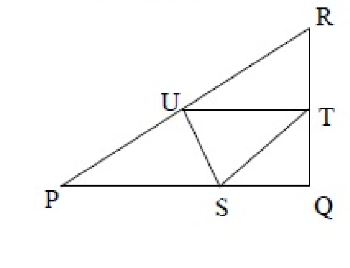
\includegraphics[width=0.6\textwidth]{1.png} 
      \caption{}
    \label{fig:fig1} 
\end{figure}
 \hfill(GATE IN 2015)

\item Right triangle PQR is to be constructed in the xy-plane so that the Right angle is at P and line PR is parallel to the x-axis. The x and y coordinates of P, Q, and R are to be integers that satisfy the inequalities: -4 $\leq$ x $\leq$ 5 and 6 $\leq$ y $\leq$ 16. How many different triangles could be constructed with these properties?

\begin{multicols}{4}
\begin{enumerate}
\item 110
\item 1,100
\item 9,900
\item 10,000
\end{enumerate}
  \end{multicols} \hfill(GATE IN 2015)

\item A coin is tossed thrice. Let X be the event that head occurs in each of the first two tosses. Let Y be the event that a tail occurs on the third toss. Let Z be the event that two tails occur in three tosses. Based on the above information, which one of the following statements is TRUE?

\begin{multicols}{2}
\begin{enumerate}
\item X and Y are not independent
\item Y and Z are dependent
\item Y and Z are independent
\item X and Z are independent
\end{enumerate}
  \end{multicols} \hfill(GATE IN 2015)

\item Let A be an n$\times$ n matrix with rank r $(0 < r < n)$. Then Ax = 0 has p independent solutions, where p is

\begin{multicols}{4}
\begin{enumerate}
\item r
\item n
\item n - r
\item n + r
\end{enumerate}
  \end{multicols} \hfill(GATE IN 2015)

\item The value of $\oint \frac{1}{z^2} dz$, where the contour is the unit circle traversed clockwise, is

\begin{multicols}{4}
\begin{enumerate}
\item -2$\pi$i
\item 0
\item 2$\pi$i
\item 4$\pi$i
\end{enumerate}
  \end{multicols} \hfill(GATE IN 2015)

\item The double integral $\int_0^a \int_x^y f(x,y)  dx  dy$ is equivalent to

\begin{multicols}{2}
\begin{enumerate}
\item $\int_0^x \int_y^y f(x,y)  dx  dy$
\item $\int_0^a \int_x^y f(x,y)  dx  dy$
\item $\int_0^a \int_x^a f(x,y)  dy  dx$
\item $\int_0^a \int_0^a f(x,y)  dx  dy$
\end{enumerate}
  \end{multicols} \hfill(GATE IN 2015)

\item The magnitude of the directional derivative of the function $f(x,y) = x^2 + 3y^2$ in a direction normal to the circle $x^2 + y^2 = 2$, at the point (1,1), is

\begin{multicols}{4}
\begin{enumerate}
\item $4\sqrt{2}$
\item $5\sqrt{2}$
\item $7\sqrt{2}$
\item $9\sqrt{2}$
\end{enumerate}
  \end{multicols} \hfill(GATE IN 2015)

\item The figure shows a half-wave rectifier circuit with input voltage $V(t) = 10 \sin (100 \pi t)$ volts. Assuming ideal diode characteristics with zero forward voltage drop and zero reverse current, the average power consumed in watts by the load resistance $R_L$ is \_\_\_\_\_ W.
\begin{figure}[H]
    \centering
      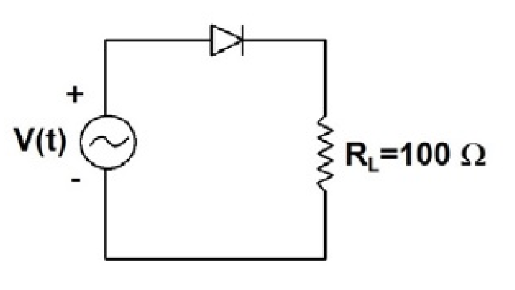
\includegraphics[width=0.6\textwidth]{2.png} 
      \caption{}
    \label{fig:fig2} 
\end{figure}
\hfill(GATE IN 2015)

\item The capacitor shown in the figure is initially charged to +10 V. The switch closes at time t = 0. Then the value of $V_C(t)$ in volts at time t = 10 ms is \_\_\_\_\_ V.
\begin{figure}[H]
    \centering
      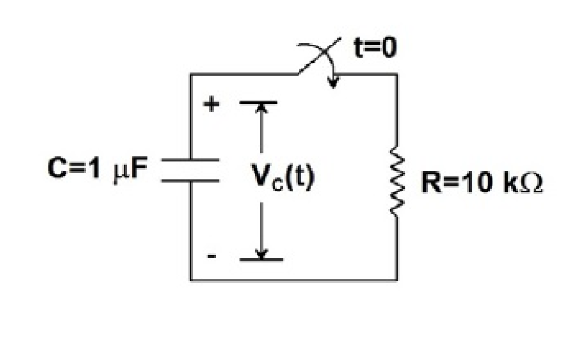
\includegraphics[width=0.6\textwidth]{3.png} 
      \caption{}
    \label{fig:fig3} 
\end{figure}
 \hfill(GATE IN 2015)

\item The torque transmitted by a cylindrical shaft is to be measured by using two strain gauges. The angles for mounting the strain gauges relative to the axis of the shaft for maximum sensitivity are

\begin{multicols}{4}
\begin{enumerate}
\item $\pm 45^\circ$
\item $\pm 60^\circ$
\item $\pm 90^\circ$
\item $\pm 180^\circ$
\end{enumerate}
  \end{multicols} \hfill(GATE IN 2015)

\item A p-type semiconductor strain gauge has a nominal resistance of 1000 $\Omega$ and a gauge factor of +200 at 25°C. The resistance of the strain gauge in ohms when subjected to a strain of +$10^{-4} m/m$  at the same temperature is --------- $\ohm$.

 \hfill(GATE IN 2015)

\item Liquid flow rate is measured using

\begin{multicols}{2}
\begin{enumerate}
\item a Pirani gauge
\item a pyrometer
\item an orifice plate
\item a Bourdon tube
\end{enumerate}
  \end{multicols} \hfill(GATE IN 2015)

\item The output voltage of the ideal transformer with the polarities and dots shown in the figure is given by
\begin{figure}[H]
    \centering
      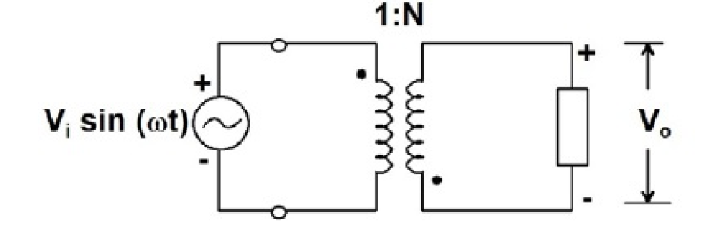
\includegraphics[width=0.6\textwidth]{4.png} 
      \caption{}
    \label{fig:fig4} 
\end{figure}
\begin{multicols}{4}
\begin{enumerate}
\item $NV_i sin \omega t$
\item $-NV_i sin\omega t$
\item $\frac{1}{N} V_i sin\omega t$
\item $-\frac{1}{N} V_i sin\omega t$
\end{enumerate}
  \end{multicols} \hfill(GATE IN 2015)

\item A load resistor$R_1$ is connected to a battery of voltage E with internal resistance$R_i$ through a resistance$R_s$ as shown in the figure. For fixed values of$R_1$ and$R_i$, the value of$R_s\geq0$ for maximum power transfer to$R_1$ is
\begin{figure}[H]
    \centering
      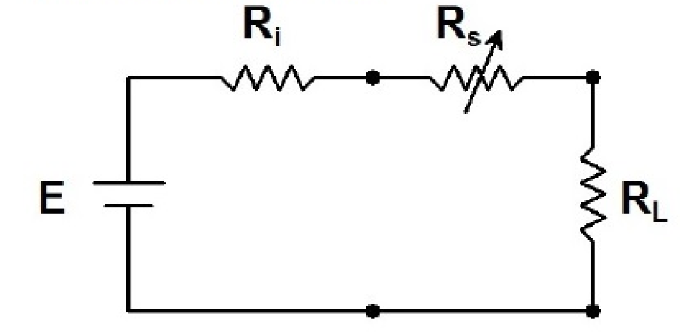
\includegraphics[width=0.6\textwidth]{5.png} 
      \caption{}
    \label{fig:fig5} 
\end{figure}
\begin{multicols}{4}
\begin{enumerate}
\item 0
\item$R_L$ -$R_i$
\item$R_L$
\item$R_L$ +$R_i$
\end{enumerate}
  \end{multicols} \hfill(GATE IN 2015)

\item Consider the logic circuit with input signal TEST shown in the figure. All gates in the figure shown have identical non-zero delay. The signal TEST which was at logic LOW is switched to logic HIGH and maintained at logic HIGH. The output
\begin{figure}[H]
    \centering
      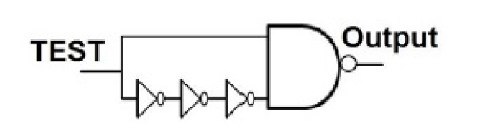
\includegraphics[width=0.6\textwidth]{6.png} 
      \caption{}
    \label{fig:fig6} 
\end{figure}
\begin{enumerate}
\item stays HIGH throughout
\item stays LOW throughout
\item pulses from LOW to HIGH to LOW
\item pulses from HIGH to LOW to HIGH
\end{enumerate}
\hfill(GATE IN 2015)

\item The logic evaluated by the circuit at the output is
\begin{figure}[H]
    \centering
      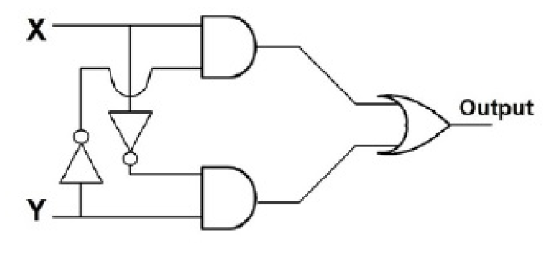
\includegraphics[width=0.6\textwidth]{7.png} 
      \caption{}
    \label{fig:fig7} 
\end{figure}
\begin{multicols}{4}
\begin{enumerate}
\item $X\overline{Y} + Y\overline{X}$
\item $\overline{(X+Y)}XY$
\item $\overline{XY} + XY$
\item $\overline{X}Y + X\overline{Y}+ X + Y$
\end{enumerate}
  \end{multicols} \hfill(GATE IN 2015)

\item In the circuit shown, the switch is momentarily closed and then opened. Assuming the logic gates to have equal non-zero delay, at steady state, the logic states of X and Y are
\begin{figure}[H]
    \centering
      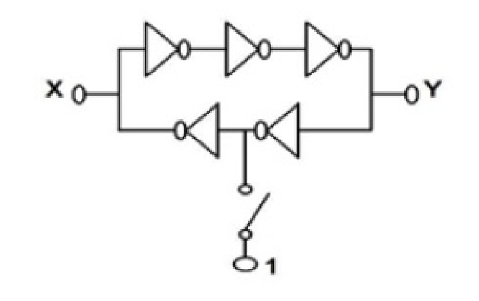
\includegraphics[width=0.6\textwidth]{8.png} 
      \caption{}
    \label{fig:fig8} 
\end{figure}
\begin{multicols}{2}
\begin{enumerate}
\item X is latched, Y toggles continuously
\item X and Y are both latched
\item Y is latched, X toggles continuously
\item X and Y both toggle continuously
\end{enumerate}
  \end{multicols} \hfill(GATE IN 2015)

\item The highest frequency present in the signal x(t) is $f_{\max}$. The highest frequency present in the signal $y(t) = x^2(t)$ is

\begin{multicols}{4}
\begin{enumerate}
\item $\frac{1}{f_{\text{max}}}$
\item $f_{\text{max}}$
\item $2f_{\text{max}}$
\item $4f_{\text{max}}$
\end{enumerate}
  \end{multicols} \hfill(GATE IN 2015)

\item The filter whose transfer function is of the form $G(s) = \frac{s^2 - bs + c}{s^2 + bs + c}$ is

\begin{multicols}{2}
\begin{enumerate}
\item a high-pass filter
\item a low-pass filter
\item an all-pass filter
\item a band-reject filter
\end{enumerate}
  \end{multicols} \hfill(GATE IN 2015)

\item Let $3 + 4j$ be a zero of a fourth order linear-phase FIR filter. The complex number which is NOT a zero of this filter is

\begin{multicols}{4}
\begin{enumerate}
\item $3-4j$
\item $\frac{3}{25} + \frac{4}{25}j$
\item $\frac{3}{25} - \frac{4}{25}j$
\item $\frac{1}{3} - \frac{1}{4}j$
\end{enumerate}
  \end{multicols} \hfill(GATE IN 2015)

\item Consider the ammeter-voltmeter method of determining the value of the resistance R using the circuit shown in the figure. The maximum possible errors of the voltmeter and ammeter are known to be 1\% and 2\% of their readings, respectively. Neglecting the effects of meter resistances, the maximum possible percentage error in the value of R determined from the measurements, is \_\_\_\_\_\%.
\begin{figure}[H]
    \centering
      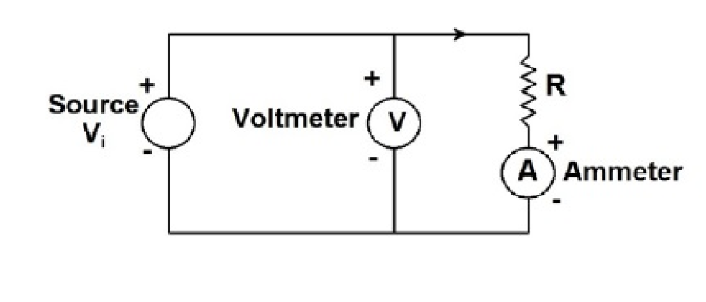
\includegraphics[width=0.6\textwidth]{9.png} 
      \caption{}
    \label{fig:fig9} 
\end{figure}
   \hfill(GATE IN 2015)

\item The bridge most suited for measurement of a four-terminal resistance in the range of 0.001 $\ohm$ to 0.1 $\ohm$ is

\begin{multicols}{2}
\begin{enumerate}
\item Wien's bridge
\item Kelvin double bridge
\item Maxwell's bridge
\item Schering bridge
\end{enumerate}
  \end{multicols} \hfill(GATE IN 2015)

\item A power line is coupled capacitively through various parasitic capacitances to a shielded signal line as shown in the figure. The conductive shield is grounded solidly at one end. Assume that the length of the signal wire extending beyond the shield, and the shield resistance are negligible. The magnitude of the noise voltage coupled to the signal line is
\begin{figure}[H]
    \centering
      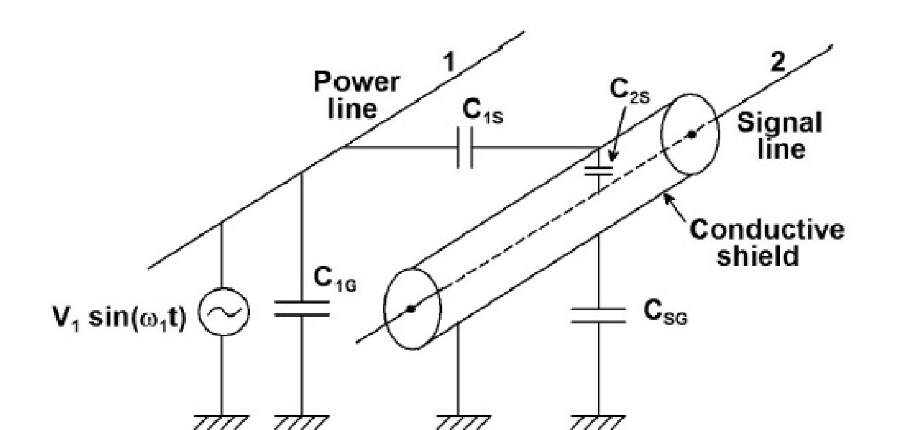
\includegraphics[width=0.6\textwidth]{10.png} 
      \caption{}
    \label{fig:fig10} 
\end{figure}
\begin{enumerate}
\item directly proportional to $C_{1G}$
\item inversely proportional to the power line frequency
\item inversely proportional to $C_{1S}$
\item zero
\end{enumerate}
 \hfill(GATE IN 2015)

\item A mass-spring-damper system with force as input and displacement of the mass as output has a transfer function $G(s) = \frac{1}{(s^2 + 24s + 900)}$. A force input F(t) = 10 sin(70t) newtons is applied at time t = 0 s. A beam from an optical stroboscope is focused on the mass. In steady state, the strobe frequency in hertz at which the mass appears to be stationary is

\begin{multicols}{4}
\begin{enumerate}
\item $\frac{5}{\pi}$
\item $\frac{15}{\pi}$
\item $\frac{35}{\pi}$
\item $\frac{50}{\pi}$
\end{enumerate}
  \end{multicols} \hfill(GATE IN 2015)

\item A system with transfer function $G(s) = \frac{1}{s^2+1}$ has zero initial conditions. The percentage overshoot in its step response is \_\_\_\_\_\%.
 \hfill(GATE IN 2015)

\item The voltage ($E_o$) developed across a glass electrode for pH measurement is related to the temperature (T) by the relation

\begin{multicols}{4}
\begin{enumerate}
\item $E_0 \propto \frac{1}{T^2}$
\item $E_0 \propto \frac{1}{T}$
\item $E_0 \propto T$
\item $E_0 \propto T^2$
\end{enumerate}
  \end{multicols} \hfill(GATE IN 2015)

\item A light detector circuit using an ideal photo-diode is shown in the figure. The sensitivity of the photo-diode is 0.5 $\mu$A/$\mu$W. With $V_r$  = 6 V, the output voltage $V_o$ = -1.0 V for 10 $\mu$W of incident light. If $V_r$ is changed to 3 V, keeping all other parameters the same, the value of $V_o$  in volts is \_\_\_\_\_ V.
\begin{figure}[H]
    \centering
      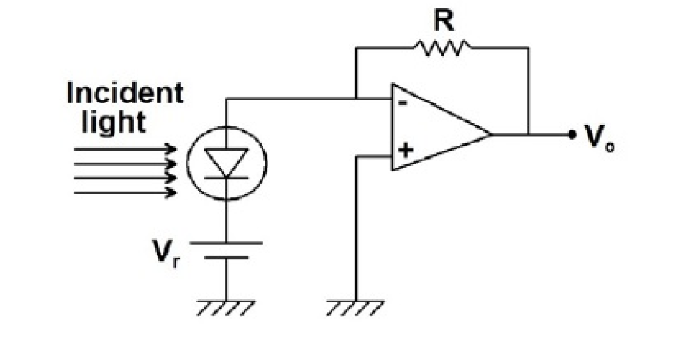
\includegraphics[width=0.6\textwidth]{11.png} 
      \caption{}
    \label{fig:fig11} 
\end{figure}
 \hfill(GATE IN 2015)

\item An apparatus to capture ECG signals has a filter followed by a data acquisition system. The filter best suited for this application is


\begin{enumerate}
\item low pass with cutoff frequency 200 Hz
\item high pass with cutoff frequency 200 Hz
\item band pass with lower and upper cutoff frequencies 100 Hz and 200 Hz for its pass band
\item band reject with lower and upper cutoff frequencies 1 Hz and 200 Hz for its stop band
\end{enumerate}
\hfill(GATE IN 2015)

\item The probability that a thermistor randomly picked up from a production unit is defective is 0.1. The probability that out of 10 thermistors randomly picked up, 3 are defective is

\begin{multicols}{4}
\begin{enumerate}
\item 0.001
\item 0.057
\item 0.107
\item 0.3
\end{enumerate}
  \end{multicols} \hfill(GATE IN 2015)

\item The probability density function of a random variable X is $p_X(x) = e^{-x}$ for $X\geq0$ and 0 otherwise. The expected value of the function ${g_X}(x) = e^{3x/4}$ is $\_\_\_\_\_$.

 \hfill(GATE IN 2015)

\item The z-transform of $x[n] = \alpha^{|n|}, 0 < |\alpha| < 1$, is X(z). The region of convergence of X(z) is

\begin{multicols}{4}
\begin{enumerate}
\item $|\alpha| < |z| < \frac{1}{|\alpha|}$
\item $|z| > \alpha$
\item $|z| > \frac{1}{|\alpha|}$
\item $|z| < \min[|\alpha|, \frac{1}{|\alpha|}]$
\end{enumerate}
  \end{multicols} \hfill(GATE IN 2015)

\item The current in amperes through the resistor R in the circuit shown in the figure is \_\_\_\_\_ A.
\begin{figure}[H]
    \centering
      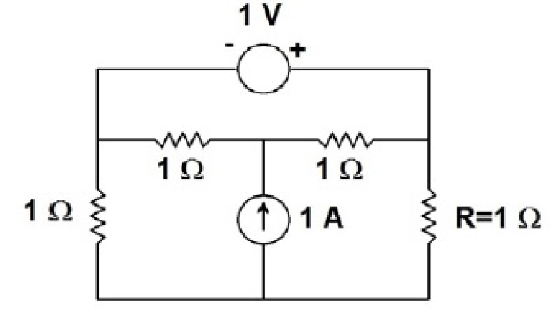
\includegraphics[width=0.6\textwidth]{12.png} 
      \caption{}
    \label{fig:fig12} 
\end{figure}
\hfill(GATE IN 2015)

\item The linear I-V characteristics of 2-terminal non-ideal dc sources X and Y are shown in the figure. If the sources are connected to a 1$\ohm$ resistor as shown, the current through the resistor in amperes is \_\_\_\_\_ A.
\begin{multicols}{2}
\begin{figure}[H]
      
\includegraphics[width=0.3\textwidth]{13.png} 
      \caption{}
    \label{fig:fig13} 
\end{figure}
\begin{figure}[H]
      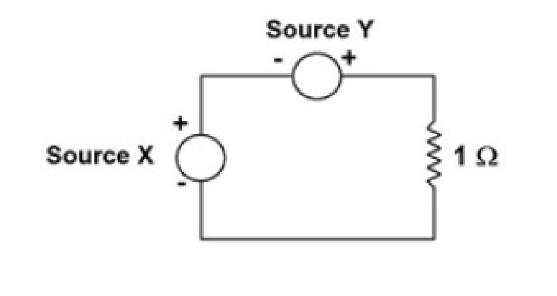
\includegraphics[width=0.3\textwidth]{14.png} 
      \caption{}
    \label{fig:fig14} 
\end{figure}
\end{multicols}
 \hfill(GATE IN 2015)

\item Consider the circuits shown in the figure. The magnitude of the ratio of the currents, i.e., $|I_1/I_2|$, is \_\_\_\_\_.
\begin{multicols}{2}
\begin{figure}[H]
      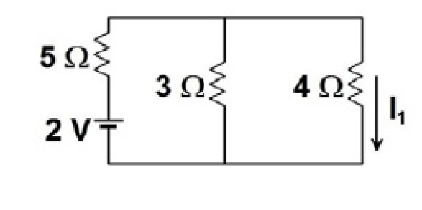
\includegraphics[width=0.3\textwidth]{15.png} 
      \caption{}
    \label{fig:fig15} 
\end{figure}
\begin{figure}[H]
      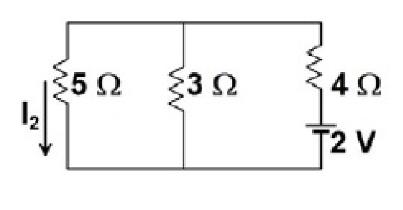
\includegraphics[width=0.3\textwidth]{16.png} 
      \caption{}
    \label{fig:fig16} 
\end{figure}
\end{multicols}
\hfill(GATE IN 2015)

\item The circuit shown in the figure is in series resonance at frequency $f_c$ Hz. The value of $V_c$ in volts is \_\_\_\_\_ V.
\begin{figure}[H]
    \centering
      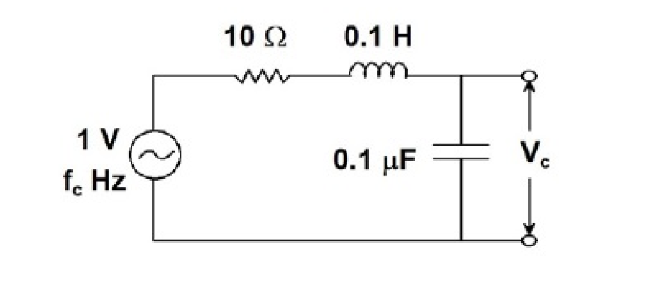
\includegraphics[width=0.6\textwidth]{17.png} 
      \caption{}
    \label{fig:fig17} 
\end{figure}
\hfill(GATE IN 2015)

\item The output frequency of an LC tank oscillator employing a capacitive sensor acting as the capacitor of the tank is 100 kHz. If the sensor capacitance increases by 10\%, the output frequency in kilohertz becomes \_\_\_\_\_ kHz.
 \hfill(GATE IN 2015)

\item The Seebeck coefficients, in $\mu$V/°C, for copper, constantan and iron, with respect to platinum, are 1.9, -38.3 and 13.3, respectively. The magnitude of the thermo emf E developed in the circuit shown in the figure, in millivolts is \_\_\_\_\_ mV.
\begin{figure}[H]
    \centering
      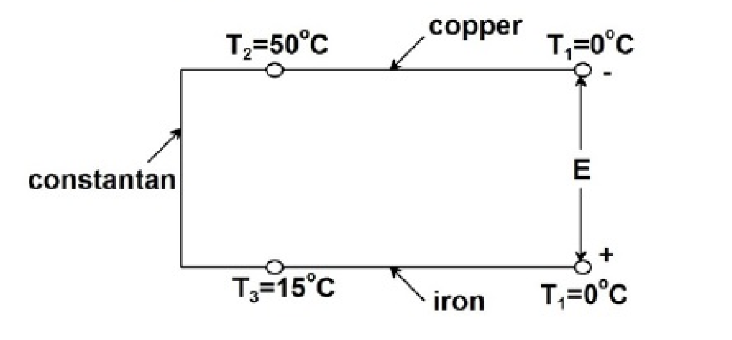
\includegraphics[width=0.6\textwidth]{18.png} 
      \caption{}
    \label{fig:fig18} 
\end{figure}
 \hfill(GATE IN 2015)

\item In the figure shown, $R_T$ represents a resistance temperature device (RTD), whose characteristic is given by $R_T = R_0(1 + \alpha T)$, where $R_o$= 100$\omega$, $\alpha$ = 0.0039 ${\degree C}^\text{-1}$ and T denotes the temperature in$\degree C$. Assuming the opamp to be ideal, the value of $V_0$ in volts when T = 100$\degree C$, is \_\_\_\_\_ V.
\begin{figure}[H]
    \centering
      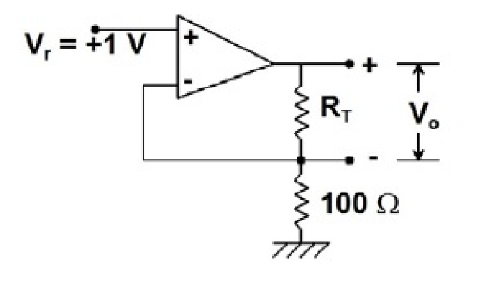
\includegraphics[width=0.6\textwidth]{19.png} 
      \caption{}
    \label{fig:fig19} 
\end{figure}
 \hfill(GATE IN 2015)

\item In the circuit shown in the figure, it is found that $V_{BE} = 0.7 V$ and $V_E = 0 V$. If $\beta_{dc} = 99$ for the transistor, then the value of $R_B$ in kilo ohms is \_\_\_\_\_ k$\Omega$.
\begin{figure}[H]
    \centering
      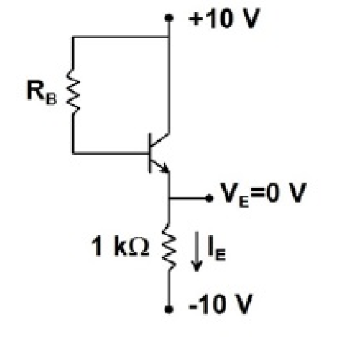
\includegraphics[width=0.6\textwidth]{20.png} 
      \caption{}
    \label{fig:fig20} 
\end{figure}
 \hfill(GATE IN 2015)

\item An opamp has ideal characteristics except that its open loop gain is given by the expression $A_V(s) = 10^4/(1 + 10^\text{-3}s)$. This op-amp is used in the circuit shown in the figure. The 3-dB bandwidth of the circuit, in rad/s, is
\begin{figure}[H]
    \centering
      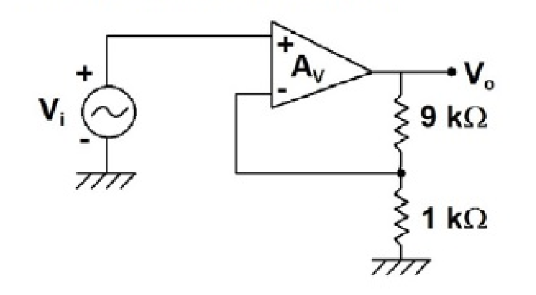
\includegraphics[width=0.6\textwidth]{21.png} 
      \caption{}
    \label{fig:fig21} 
\end{figure}
\begin{multicols}{4}
\begin{enumerate}
\item $10^2$
\item $10^3$
\item $10^4$
\item $10^6$
\end{enumerate}
  \end{multicols} \hfill(GATE IN 2015)

\item In the circuit shown, the voltage source V(t) = 15 + 0.1 sin(100t) volts. The PMOS transistor is biased such that it is in saturation with its gate-source capacitance being 4 nF and its transconductance at the operating point being 1 mA/V. Other parasitic impedances of the MOSFET may be ignored. An external capacitor of capacitance 2 nF is connected across the PMOS transistor as shown. The input impedance in mega ohm as seen by the voltage source is \_\_\_\_\_ M$\Omega$.
\begin{figure}[H]
    \centering
      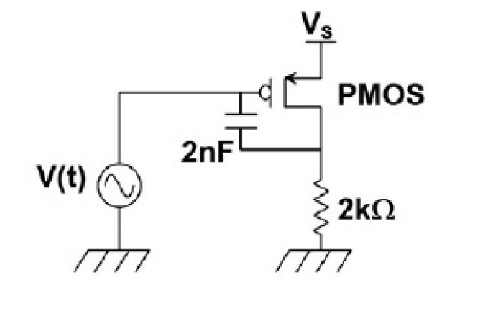
\includegraphics[width=0.6\textwidth]{22.png} 
      \caption{}
    \label{fig:fig22} 
\end{figure}
 \hfill(GATE IN 2015)

\item An ADC is interfaced with a microprocessor as shown in the figure. All signals have been indicated with typical notations. Acquisition of one new sample of the analog input signal by the microprocessor involves
\begin{figure}[H]
    \centering
      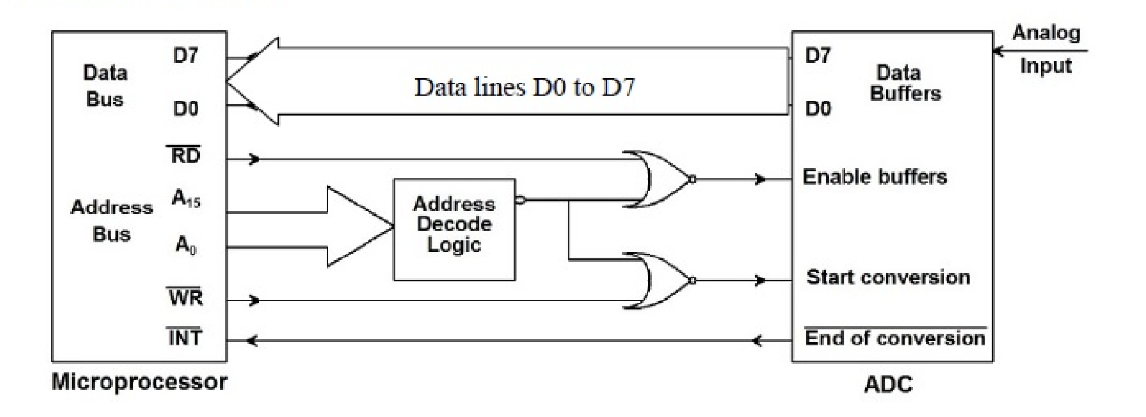
\includegraphics[width=0.6\textwidth]{23.png} 
      \caption{}
    \label{fig:fig23} 
\end{figure}
\begin{enumerate}
\item one READ cycle only
\item one WRITE cycle only
\item one WRITE cycle followed by one READ cycle
\item one READ cycle followed by one WRITE cycle
\end{enumerate}
\hfill(GATE IN 2015)

\item The number of clock cycles for the duration of an input pulse is counted using a cascade of N decade counters (DC 1 to DC N) as shown in the figure. If the clock frequency in mega hertz is f, the resolution and range of measurement of input pulse width, both in $\mu$s, are respectively,
\begin{figure}[H]
    \centering
      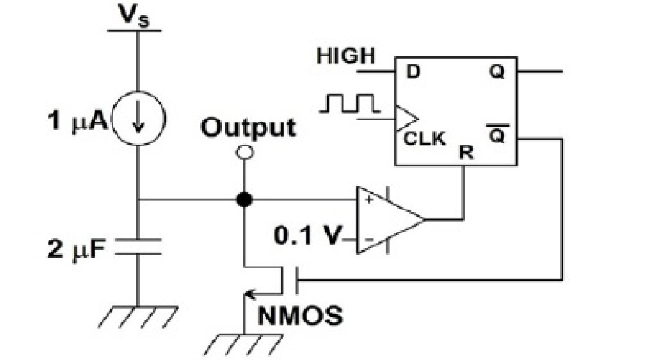
\includegraphics[width=0.6\textwidth]{24.png} 
      \caption{}
    \label{fig:fig24} 
\end{figure}
\begin{multicols}{4}
\begin{enumerate}
\item $\frac{1}{f}$ and $\frac{(2^N - 1)}{f}$
\item $\frac{1}{f}$ and $\frac{(10^N - 1)}{f}$
\item $\frac{10^N}{f}$ and $\frac{(10^N - 1)}{f}$
\item $\frac{2^N}{f}$ and $\frac{(2^N - 1)}{f}$
\end{enumerate}
  \end{multicols} \hfill(GATE IN 2015)

\item For the circuit shown in the figure, the rising edge triggered D-flip flop with asynchronous reset has a clock frequency of 1 Hz. The NMOS transistor has an ON resistance of 1000$\omega$ and an OFF resistance of infinity. The nature of the output waveform is
\begin{figure}[H]
    \centering
      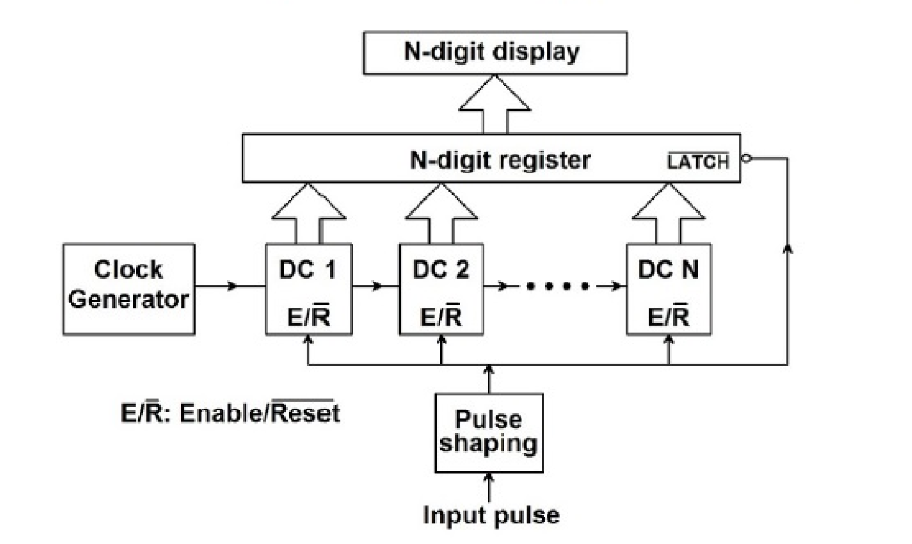
\includegraphics[width=0.6\textwidth]{25.png} 
      \caption{}
    \label{fig:fig25} 
\end{figure}
\begin{figure}[H]
    \centering
      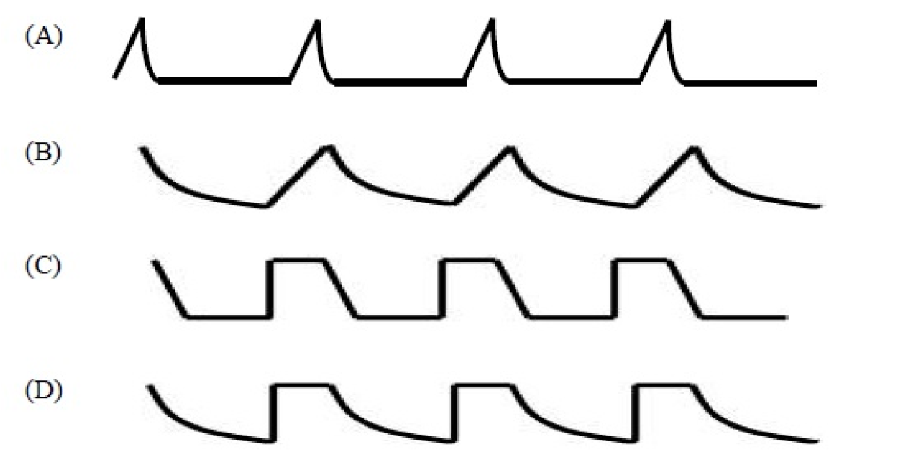
\includegraphics[width=0.6\textwidth]{26.png} 
      \caption{}
    \label{fig:fig26} 
\end{figure}
 \hfill(GATE IN 2015)

\item A transfer function G(s) with the degree of its numerator polynomial zero and the degree of its denominator polynomial two has a Nyquist plot shown in the figure. The transfer function represents
\begin{figure}[H]
    \centering
      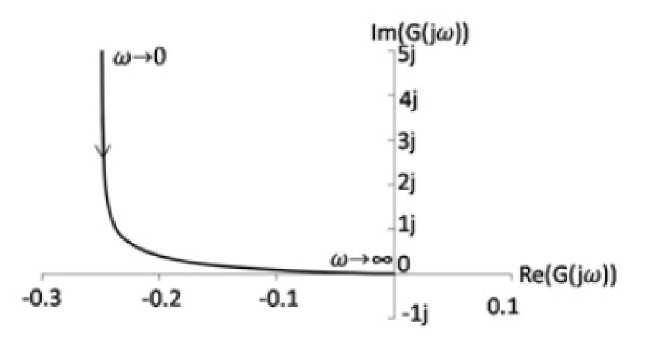
\includegraphics[width=0.6\textwidth]{27.png} 
      \caption{}
    \label{fig:fig27} 
\end{figure}
\begin{multicols}{2}
\begin{enumerate}
\item a stable, type-0 system
\item a stable, type-1 system
\item an unstable, type-0 system
\item an unstable, type-1 system
\end{enumerate}
  \end{multicols} \hfill(GATE IN 2015)

\item In the circuit shown in the figure, both the NMOS transistors are identical with their threshold voltages being 5 V. Ignoring channel length modulation, the output voltage $V_{out}$ in volt is \_\_\_\_\_ V.
\begin{figure}[H]
    \centering
      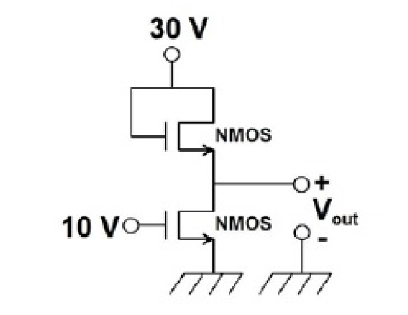
\includegraphics[width=0.6\textwidth]{28.png} 
      \caption{}
    \label{fig:fig28} 
\end{figure}
 \hfill(GATE IN 2015)

\item The signal x[n] = sin($\pi$n/6)/($\pi$n) is processed through a linear filter with the impulse response $h[n] = sin(\omega_c n)/(\pi n)$ where $\omega_c > \pi/6$. The output of the filter is

\begin{multicols}{2}
\begin{enumerate}
\item sin(2$\omega_c$ n)/($\pi$n)
\item sin($\pi$n/3)/($\pi$n)
\item $[sin(\pi n/6)/(\pi n)]^2$
\item sin($\pi$n/6)/($\pi$n)
\end{enumerate}
  \end{multicols} \hfill(GATE IN 2015)

\item A signal is band-limited to 0 to 12 kHz. The signal spectrum is corrupted by additive noise which is band-limited to 10 to 12 kHz. Theoretically, the minimum rate in kilohertz at which the noisy signal must be sampled so that the UNCORRUPTED PART of the signal spectrum can be recovered, is \_\_\_\_\_ kHz.

 \hfill(GATE IN 2015)

\item Consider a low-pass filter module with a pass-band ripple of $\delta$ in the gain magnitude. If M such identical modules are cascaded, ignoring the loading effects, the pass-band ripple of the cascade is

\begin{multicols}{4}
\begin{enumerate}
\item $1 - (1 - \delta)^M$
\item $\delta^M$
\item $(1 - \delta^M)$
\item $(1 - \delta)^M$
\end{enumerate}
  \end{multicols} \hfill(GATE IN 2015)

\item The fundamental period of the signal x(t) = 2 cos(2$\pi$t/3) + cos($\pi$t), in seconds, is \_\_\_\_\_ s.

\hfill(GATE IN 2015)

\item If the deflection of the galvanometer in the bridge circuit shown in the figure is zero, then the value of $R_x$ in ohms is \_\_\_\_\_ $\ohm$.
\begin{figure}[H]
    \centering
      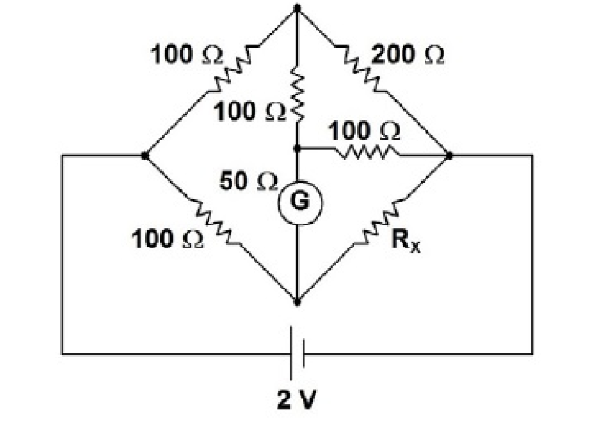
\includegraphics[width=0.6\textwidth]{29.png} 
      \caption{}
    \label{fig:fig29} 
\end{figure}
 \hfill(GATE IN 2015)

\item In the potentiometer circuit shown in the figure, the expression for $V_x$ is
\begin{figure}[H]
    \centering
      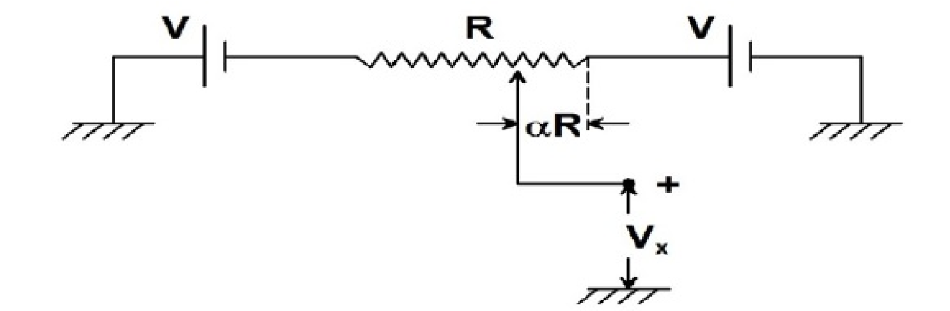
\includegraphics[width=0.6\textwidth]{30.png} 
      \caption{}
    \label{fig:fig30} 
\end{figure}
\begin{multicols}{4}
\begin{enumerate}
\item (1 - 2$\alpha$) V
\item (1 - $\alpha$) V
\item ($\alpha$ - 1) V
\item $\alpha$ V
\end{enumerate}
  \end{multicols} \hfill(GATE IN 2015)

\item The open loop transfer function of a system is G(s) = $(s^2 + 6s + 10)/(s^2 + 2s + 2)$. The angles of arrival of its root loci are

\begin{multicols}{4}
\begin{enumerate}
\item ±$\pi$/4
\item ±$\pi$/3
\item ±$\pi$/2
\item ±5$\pi$/6
\end{enumerate}
\end{multicols} \hfill(GATE IN 2015)

\item A system is represented in state-space as $\dot{X} = Ax + Bu$, where $\Vec{A} = \myvec{ 1 & 2 \\ a & 6 }$ and $\Vec{B} = \myvec{ 1 \\ 1 }$. The value of a for which the system is not controllable is \_\_\_\_\_.

 \hfill(GATE IN 2015)

\item A liquid level measurement system employing a radio-isotope is mounted on a tank as shown in the figure. The absorption coefficient of water for the radiation is 7.7 $m^\text{-1}$. If the height of water in the tank is reduced from 100 mm to 90 mm, the percentage change in the radiation intensity received by the detector, neglecting absorption of the radiation by air, is \_\_\_\_\_\%.
\begin{figure}[H]
    \centering
      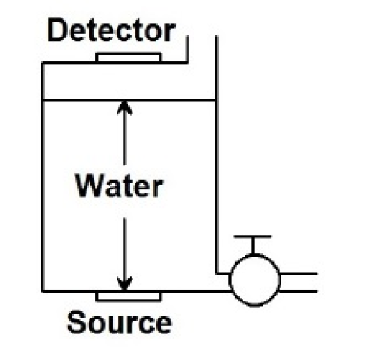
\includegraphics[width=0.6\textwidth]{31.png} 
      \caption{}
    \label{fig:fig31} 
\end{figure}
 \hfill(GATE IN 2015)

\item The figure shows a spot of light of uniform intensity 50 W/m² and size 10 mm$\times$ 10 mm incident at the exact center of a photo-detector, comprising two identical photo-diodes $D_1$ and $D_2$. Each diode has a sensitivity of 0.4 A/W and is operated in the photoconductive mode. If the spot of light is displaced upwards by 100 $\mu$m, the resulting difference between the photocurrents generated by $D_1$ and $D_2$ in micro amperes, is \_\_\_\_\_ $\mu$A.
\begin{figure}[H]
    \centering
      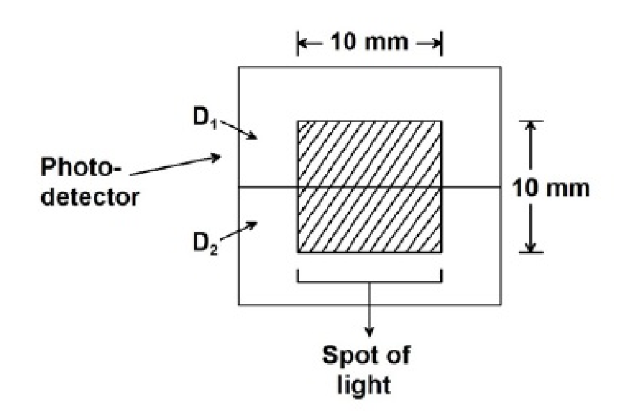
\includegraphics[width=0.6\textwidth]{32.png} 
      \caption{}
    \label{fig:fig32} 
\end{figure}
 \hfill(GATE IN 2015)

\item A beam of monochromatic light passes through two glass slabs of the same geometrical thickness at normal incidence. The refractive index of the first slab is 1.5 and that of the second, 2.0. The ratio of the time of passage of the beam through the first to the second slab is \_\_\_\_\_.

 \hfill(GATE IN 2015)

\item The resolving power of a spectrometer consisting of a collimator, a grating and a telescope can be increased by


\begin{enumerate}
\item increasing the angular magnification of the telescope
\item increasing the period of the grating
\item decreasing the period of the grating
\item decreasing the slit-width of the collimator
\end{enumerate}
\hfill(GATE IN 2015)
\end{enumerate}
\end{document}
